\documentclass[conference]{IEEEtran}

\makeatletter
% IEEEtran.cls defines \labelindent for backward compatibility reasons
% Undefine \labelindent to allow the use of package enumitem
\let\labelindent\relax
\makeatother

\usepackage[utf8]{inputenc}
\usepackage[T1]{fontenc}
\usepackage{microtype}

\usepackage{array}
\usepackage{balance}
\usepackage{booktabs}
\usepackage{cite}
\usepackage{color}
\usepackage{comment}
\usepackage{enumitem}
\usepackage[para]{footmisc}
\usepackage{framed}
\usepackage[pdftex]{graphicx}
\usepackage{listings}
\usepackage{subcaption}
\usepackage{url}


% SQUEEZE
%\addtolength{\parskip}{-1pt}


\definecolor{lightred}{RGB}{150,0,0}
\definecolor{lightgreen}{RGB}{0,150,0}
\definecolor{lightblue}{RGB}{0,0,150}

\lstdefinelanguage{diff}{
  morecomment=[f][\color{lightblue}]{diff },
  morecomment=[f][\color{lightblue}]{index },
  morecomment=[f][\color{lightblue}]{@@},     % group identifier
  morecomment=[f][\color{lightred}]-,         % deleted lines
  morecomment=[f][\color{lightgreen}]+,       % added lines
  morecomment=[f][\color{lightblue}]{---},    % Diff header lines (must appear after +,-)
  morecomment=[f][\color{lightblue}]{+++},
}
\hyphenation{}

\newcommand{\attn}[1]{{\color{red}#1}}
\newcommand{\desc}[1]{{\emph{\color{blue}#1}}}
\newcommand{\needcite}{\attn{\tiny{[cite]}}}
\newcommand{\todo}[1]{\strut\smash{\colorbox{yellow}{\bf TODO: #1}}}

\begin{document}
\title{Modeling Changeset Topics for Feature Location}
\author{
    \IEEEauthorblockN{
        Christopher S.\ Corley,
        Kelly L.\ Kashuda
    }
    \IEEEauthorblockA{
        The University of Alabama\\
        Tuscaloosa, AL, USA\\
        \{cscorley, klkashuda\}@ua.edu
    }

    \and

    \IEEEauthorblockN{
        Nicholas A.\ Kraft
    }
    \IEEEauthorblockA{
        ABB Corporate Research\\
        Raleigh, NC, USA\\
        nicholas.a.kraft@us.abb.com
    }
}


\maketitle

\begin{abstract}
Feature location is a program comprehension activity in which a developer
inspects source code to locate the classes or methods that implement a feature of interest.
Many feature location techniques (FLTs) are based on text retrieval models, and
in such FLTs it is typical for the models to be trained on source code snapshots.
However, source code evolution leads to model obsolescence and
thus to the need to retrain the model from the latest snapshot.
In this paper, we introduce a topic-modeling-based FLT in which the model
is built incrementally from source code history.
By training an online learning algorithm using changesets, the FLT
maintains an up-to-date model without incurring the non-trivial computational cost associated with retraining traditional FLTs.
Overall, we studied over 1,200 defects and features from 14 open-source Java projects.
We also present a historical simulation that demonstrates how the FLT performs as a project evolves.
Our results indicate that the accuracy of a changeset-based FLT is similar to that of a snapshot-based FLT, but without the retraining costs.
\end{abstract}

\begin{IEEEkeywords}
program comprehension;
feature location;
topic modeling;
mining software repositories;
changesets
\end{IEEEkeywords}

\section{Introduction}
\label{sec:intro}
% vim:syntax=tex

Software developers are often confronted with maintenance tasks that involve navigation of repositories that preserve vast amounts of project history.
Navigating these software repositories can be a time-consuming task, because their organization can be difficult to understand.
A software developer who is tasked with changing a large software system spends effort on program comprehension activities to gain the knowledge needed to make the change~\cite{Corbi:1989}.
Fortunately, topic models such as
latent semantic indexing (LSI)~\cite{Deerwester-etal:1990} and
latent Dirichlet allocation (LDA)~\cite{Blei-etal:2003}
can help developers to navigate and understand software repositories
by discovering topics (word distributions) that reveal the thematic structure
of the data~\cite{Linstead-etal:2007,Thomas-etal:2011,Hindle-etal:2012}.

One particular application of topic models is for \emph{feature location}.
Feature location is the act of identifying the source code that implements a system feature.
The current state-of-the-practice for feature location is to use a keyword search tool, such as \texttt{grep}.
However, Ko et al.~\cite{Ko-etal:2006} show that developers fail using this type of searching upwards to 88\% of the time. 
Information retrieval techniques, such as topic modeling, show promise in remedying this problem~\cite{Marcus-etal:2004}.

Typical topic-model-based feature location techniques (FLT) construct models from corpora of text extracted from a source code snapshot~\cite{Dit-etal:2013b}.
To use a topic-model-based FLT, there are generally two key steps: training and indexing.
In the first step, a corpus of source code entities, such as methods or classes, are used to train the model to learn word co-occurences within those entities.
The indexing step uses the trained model to construct an index of the source code entities based on their inferred topic distribution.
Keeping such a model up-to-date is expensive, because the frequency and scope of source code changes, such as method removal, necessitate retraining the model on the updated corpus.
This situation is sub-optimal whether your perspective is academic research or industrial tool-building.
An optimal topic model is one that does not incur this computational cost to stay up-to-date.

In this paper, we propose a fresh take on topic-modeling-based FLTs by leveraging online topic models and mining software repositories to construct topic models that do not need retraining.
Online topic models do not need to know the entire input corpus prior to training~\cite{Hoffman-etal:2010,Radim:2011}.
That is, online topic models can be instantiated once and incrementally updated over time.
% Additionally, training the model and infering how documents relate with the model can be intermixed.
Moreover, a version control repository, such as Git, keeps a history of source code documents as they change over time.
These changes are represented as changesets, which provide concise views of the differences between two revisions of the same document.
By training an online topic model on changesets and indexing the source code on that model, we can stream documents (i.e., changesets) from the version control repository to the topic model.
This enables searching over the current source code index without retraining an entirely new model.

In our previous work~\cite{Corley-etal:2014}, we show that topic models trained on changesets produce topics which have comparable
topic distinctness scores~\cite{Thomas-etal:2011} as topic models trained on snapshots.
We expand the work to demonstrate the effectiveness of changeset topic modeling for feature location and report on an empirical study in which we investigate the feasibility of this approach.
We define two topic-model-based FLTs on both LSI and LDA using changesets.
We combine two benchmarks totaling over 1200 defects and features from fourteen open source Java projects.
We also present a \emph{temporal simulation} in which we approximate how the FLT would perform throughout the evolution of a project.

Our results show that the changeset approach is feasible and practical.
In many cases the changeset approach out-performs current snapshot approaches, but is no silver bullet to in defeating snapshot-based approaches.
However, the performance in both the failing and succeeding cases are comparable.
Hence, we argue that the changeset-based topic modeling warrants further investigation.

% blah
We also show that evalutating an FLT in a temporally-aware manner improves the performance of the FLT.
That is, rather than training a topic model on the entire corpus at once,
we train it on only the changes that occur within the time window between features in the benchmarks.

This paper makes the following contributions:

\begin{itemize}
    \item An approach using changesets for feature location
    \item A empirical study of fourteen open source Java projects
    \item An updated dataset of systems used in this study
    \item Finally, towards increasing open science principles in software engineering:
        the complete project history, source code, and data for replication of this study.
\end{itemize}

The remainder of the paper is organized as follows.
We first review background and related work (\S\ref{sec:related})
before introducing our new changeset-based FLT (\S\ref{sec:changeset}).
We next discuss our case study (\S\ref{sec:study}), which spans fourteen open source Java projects.
We then conclude (\S\ref{sec:conclusion}).



\section{Background \& Related Work}
\label{sec:related}
% vim:syntax=tex


In this section, we review background material of the document extraction and retrieval process
typically used on snapshot-based FLTs,
and review related work on topic modeling and feature location.

\subsection{Document Extraction and Retrieval Process}

\begin{figure*}
\centerline{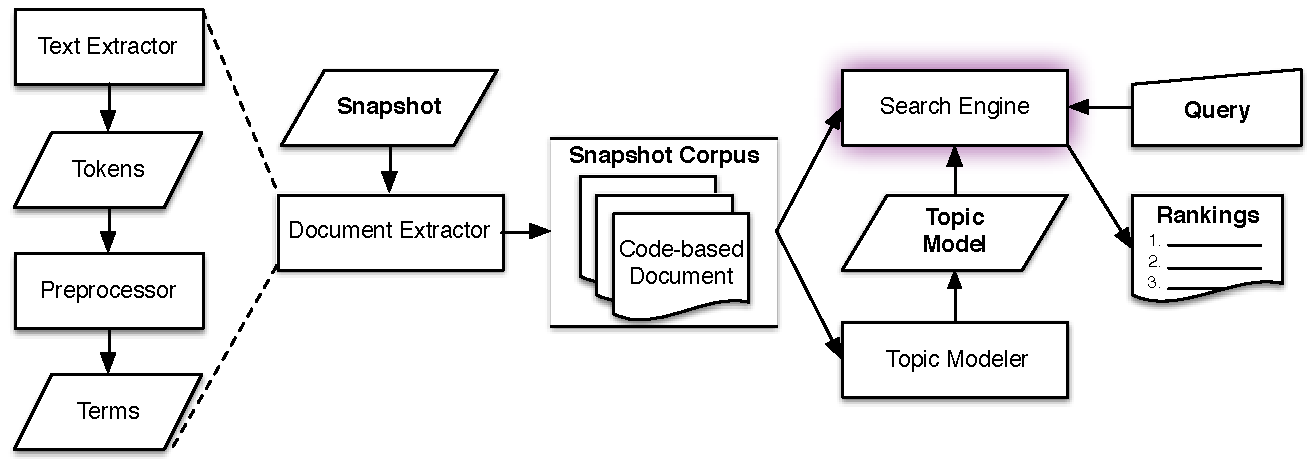
\includegraphics[width=.75\textwidth]{figures/snapshot-flt}}
\caption{Feature location using snapshots}
\label{fig:snapshot}
\end{figure*}

We use the following terminology to describe document extraction of source code.
A \textit{word} is the basic unit of discrete data in a software lexicon and is a sequence of letters.
A \textit{token} is a sequence of non-whitespace characters containing one or more words.
An \textit{entity} is a named source element such as a method,
and an \textit{identifier} is a token representing the name of an entity.
\textit{Comments} and \textit{literals} are sequences of tokens delimited by language-specific markers (e.g., /* */ and quotes).
The \textit{document} which corresponds to a class is a sequence of words $d = (w_1, \ldots, w_m)$,
and a \textit{corpus} is a set of documents (i.e., classes) $D = (d_1, \ldots, d_n)$.

The left side of Figure~\ref{fig:snapshot} illustrates the document extraction process.
A document extractor takes source code as input and produces a corpus as output.
Each document in the corpus contains the words associated with a source code entity
such as a class or method.
The text extractor is the first part of the document extractor.
It parses the source code and produces a token stream for each class.
The preprocessor is the second part of the document extractor.
It applies a series of transformations to each token and
produces one or more words from the token.
The transformations~\cite{Marcus-etal:2004,Marcus-Menzies:2010}: % that we use are:
\begin{itemize}
    \item {\it Splitting}: separate tokens into constituent words
        based on common coding style conventions (e.g., the use of camel case or underscores)
        and on the presence of non-letters (e.g., punctuation or digits)
    \item {\it Normalizing}: replace each upper case letter with the corresponding lower case letter
    \item {\it Filtering}: remove common words such as articles (e.g., `an' or `the'),
        programming language keywords, standard library entity names, or short words
\end{itemize}

The right side of Figure~\ref{fig:snapshot} illustrates the retrieval process.
The main prerequisite of the retrieval process is to build the search engine.
The search engine is constructed from the topic model trained from the corpus
and an index of that corpus inferred from that model, known as $\theta$.
The primary function of the search engine is to rank documents in relation to the query.
The search engine performs a pairwise classification of the query
to each document and ranks the documents based on their scores.

To accomplish the classification step using a topic model,
the search engine infers $\theta_{Snapshot}$, i.e.,
the topic-document probability distribution of each document in the snapshot corpus,
as well as $\theta_{Query}$, i.e., the topic-document probability distribution of the query.
Then a similarity measure for probability distributions, such as
cosine similarity or Hellinger distance, can be used to make pairwise comparisons
between $\theta_{Query}$ and $\theta_{Snapshot}$.
Hellinger distance ($H$) can be defined as:

\begin{equation}
    H(P, Q) = \frac{1}{\sqrt{2}} \; \sqrt{\sum_{i=1}^{k} (\sqrt{P_i} - \sqrt{Q_i})^2}
\end{equation}

where $P$ and $Q$ are two discrete probability distributions of length $k$.


\subsection{Topic Modeling}

\subsubsection{Latent Dirichlet Allocation}

Latent Dirichlet allocation~\cite{Blei-etal:2003} is a generative topic model.
LDA models each document in a corpus of discrete data as a finite mixture over
a set of topics and models each topic as an infinite mixture over a set of
topic probabilities.  That is, LDA models each document as a probability
distribution indicating the likelihood that it expresses each topic and models
each topic that it infers as a probability distribution indicating the
likelihood of a word from the corpus being assigned to the topic.

Hoffman et al.~\cite{Hoffman-etal:2010} introduce a version of LDA which is
\emph{online}.
Online LDA allows the model to be updated incrementally without needing
to know about the documents prior to model construction.
Zhai and Boyd-Graber~\cite{Zhai-Boyd-Graber:2013} introduce an extension of LDA
in which the model also does not need to know about the corpus vocabulary prior to training.

\subsubsection{Latent Semantic Indexing}

Latent semantic indexing~\cite{Deerwester-etal:1990} is an indexing and
retrieval methodology. LSI uses a statistical technique, singular value
decomposition to identify patterns within the unstructured data, identifying
relationships between terms and documents, placing documents that are related
close to one another creating a semantic space. That is, LSI estimates the
latent structure by taking each document in the corpus and forming weighted
vectors applying cosine similarity to the vectors measuring the semantic
similarities between documents~\cite{Binkley-Lawrie:2010}.
{\v R}eh{\r u}{\v r}ek~\cite{Radim:2011} outlines extensions to LSI
which enable the algorithm to be online.


\subsection{Feature Location}

A feature~\cite{Biggerstaff-etal:1993} is a visible functionality within the source code
(feature is defined weakly throughout the literature because of the vast
context in which it can be used). Feature (or concept) location is a program
comprehension technique to locate source code elements (i.e., methods)
within the source code that relate to specific functional
requirements~\cite{Eisenbarth-etal:2001, Biggers-etal:2014}. Locating functionalities
within the source code is a prerequisite for software evolution.  Identifying features is a specifically crucial and frequent task for
developers, when adding new features, modifying existing features and removing
unwanted features (e.g.  bugs)~\cite{Rajlich-Gosavi:2004, Dit-etal:2013b}. Locating bugs,
or bug localization~\cite{Lukins-etal:2008, Bassett-Kraft:2013} is analogous to removing unwanted features.

Feature location is commonly categorized as a static, dynamic or a hybrid
technique involving a combination of the two. Static feature
location~\cite{Zhao-etal:2006} is a method that statistically analyzes
static documents, or source code. This is done by manually or automatically
analyzing the text to explore the dependencies within the structure. Dynamic
feature location applies a statistical analysis to the execution trace of a
specific scenario, therefore requiring a working system~\cite{Eisenbarth-etal:2001,Poshyvanyk-etal:2007}.
Hybrid techniques~\cite{Eisenbarth-etal:2003, Eaddy-etal:2008, Revelle-etal:2010} involve a combination of a static analysis of
the source text and an analysis of scenarios in the execution trace. By
blending the two it was found that this technique was applicable to working
systems in providing higher precision for locating features~\cite{Poshyvanyk-etal:2007,
Ernst:2004, Revelle-Coppitt:UNK}. In this study, we are applying two static
techniques, an LDA-based FLT and an LSI-based FLT.

Dit et al.~\cite{Dit-etal:2013b} provide a taxonomy and survey of feature
location in source code covering the scope of FLTs.  Marcus et
al~\cite{Marcus-etal:2004} use LSI-based feature location to find concepts based on
queries from the user, and modules within the system in comparison to the
dependence graph approach. They found that concepts in the code were able to be
identified with user specified terms and identifiers as well as an easier build
process. LSI-based FLTs have been widely used by many others~\cite{
Poshyvanyk-etal:2006, Poshyvanyk-Marcus:2007, Liu-etal:2007, Scanniello-Marcus:2011,
Eaddy-etal:2008, Cubranic-etal:2005}.

Lukins et al.~\cite{Lukins-etal:2008} use an LDA-based FLT and
find that that it outperforms an LSI-based FLT.
Biggers et al.~\cite{Biggers-etal:2014} investigate the various configuration
parameters for an LDA-based FLT.
Bassett and Kraft~\cite{Bassett-Kraft:2013} find that using structural
term weighting increases the performance of an LDA-based FLT.

Antoniol and Gueheneuc~\cite{Antoniol-Gueheneuc:2005, Antoniol-Gueheneuc:2006} use a combination of dynamic and
static FLTs to improve program comprehension of large multi-threaded
object oriented systems, particularly they run this integrated technique on
Mozilla and Firefox as well as smaller systems JHotDraw, XFig, Chimera and
ICEBrowser. Taking these systems and using static analysis, they represent them
in Abstract Object Language format and then manipulate them using a meta model,
PADL that represents object oriented systems independent of the language. To
avoid the noise and imprecision of dynamic FLT they use process emulation
during the execution of scenarios assigning probabilistic ranking of features as
relevant or irrelevant. Their approach proves to minimize the amount of code
needed for program comprehension as well as providing micro-architectures of
each system.

Petrenko et al.~\cite{Petrenko-etal:2008} perform a textual search with a grep-based
feature location with ontology fragments using Eclipse and Mozilla for their
study. The ontology fragments work as a template for a query, storing the
developers' knowledge of the concept they is trying to locate, and updating the
fragments as further knowledge is gained. Wilson~\cite{Wilson:2010} extended this
study with a systematic approach, formulating the queries for grep-based search, and
directly using the ontology fragments. Four developers using the same systems
as Petrenko et al, showed that using the ontology fragments as queries, providing
only partial knowledge, was enough to accurately locate concepts within the
two systems.

Rao et al.~\cite{Rao-etal:2013} also target the problem of building
topic models, introducing an incremental framework for bug localization.
Although practical, the approach involves using an extended topic modeler to allow
updating, adding, and removing documents from the model and index post-hoc.
While the approach is essentially equivalent to topic modeling in batch,
Rao~\cite{Rao:2013} notes that these algorithm modifications have limitations and
thus models may need to be periodically retrained.


\section{Changeset Topic Modeling}
\label{sec:changeset}
% vim:syntax=tex

In this section we describe how a TM-based FLT can use changesets.

\subsection{Terminology}

In addition to the terminology described in Section~\ref{sec:related}, we use
the following terminology to describe the document extraction and retrieval
process of changesets.

A \textit{diff} is a set of text which represents the differences between two texts.
A \textit{patch} is a set of instructions (i.e., diffs) that is used to transform one set of texts into another.
\textit{Context lines} denote text useful for transforming the text, but do not represent the differences.
\textit{Added lines} are lines which were added in order to transform the first text into the second.
Similarly, \textit{removed lines} are lines which are removed for this same purpose.
A \textit{changeset}, ideally, represents a single feature modification,
addition, or deletion, which may crosscut many source code entities.
A \textit{commit} is a representation of a changeset in a version control system, such as Git or Subversion.
Figure~\ref{fig:diff} shows an example changeset from Git.


\begin{figure*}[t]
\centering
\footnotesize
\begin{lstlisting}[language=diff, basicstyle=\ttfamily]
diff --git a/src/java/net/sf/jabref/EntryEditor.java b/src/java/net/sf/jabref/EntryEditor.java
index 8c56723..6b4788e 100644
--- a/src/java/net/sf/jabref/EntryEditor.java
+++ b/src/java/net/sf/jabref/EntryEditor.java
@@ -669,7 +669,8 @@ public class EntryEditor extends JPanel implements VetoableChangeListener {
     public void storeCurrentEdit() {
         Component comp = Globals.focusListener.getFocused();
         if ((comp == source) || ((comp instanceof FieldEditor) && this.isAncestorOf(comp))) {
-            ((FieldEditor)comp).clearAutoCompleteSuggestion();
+            if (comp instanceof FieldEditor)
+                ((FieldEditor)comp).clearAutoCompleteSuggestion();
             storeFieldAction.actionPerformed(new ActionEvent(comp, 0, ""));
         }
     }
\end{lstlisting}
\caption{Example of a \texttt{git diff}.
This changeset addresses JabRef's Issue \#2904968.
Black or blue lines denote metadata about the change useful for patching.
In particular, black lines represent context lines (beginning with a single space).
Red lines (beginning with a single~\texttt{-}) denote line removals,
and green lines (beginning with a single~\texttt{+}) denote line additions.}
\label{fig:diff}
\vspace{-10pt}
\end{figure*}

\subsection{Feature location using changesets}

The overall difference in our methodology and the standard methodology described in Section~\ref{sec:snapshot-flt} is minimal.
For example, compare Figures~\ref{fig:snapshot}~and~\ref{fig:changeset}.
In the changeset approach, we only need to replace the documents on which the topic model is trained
while the remainder of the approach remains the same.
%Our work can be viewed as a hybrid of textual and historical analyses
%under the Dit et al.~\cite{Dit-etal:2011} taxonomy.
% % already mentioned elsewhere


The changeset approach requires two types of document extraction:
the snapshot of the state of source code at a commit of interest, such as
a tagged release, and every changeset in the source code history leading up to
the same commit of interest.  The left side of Figure~\ref{fig:changeset}
illustrates the dual-document extraction approach.

The document extraction process for the snapshot remains the same as covered in
Section~\ref{sec:related} while the document extractor for the changesets parses
each changeset for the removed, added, and context lines.  From there, each line
is tokenized by the text extractor.  The same preprocessor transformations as
before occur in both the snapshot and changesets.  The snapshot vocabulary is
always a subset of the changeset vocabulary~\cite{Corley-etal:2014}.

The right side of Figure~\ref{fig:changeset} illustrates the retrieval process.
The key intuition to our methodology is that a topic model such as LDA or LSI can
infer \emph{any} document's topic proportions regardless of the documents used
to train the model.  In fact, this is also what determining the topic
proportions of a user-created query relies on. Likewise, so are other unseen
documents. In our approach, the seen documents are changesets and the unseen
documents are the source code entities of the snapshot.

Hence, we train a topic model on the changeset corpus and use the model to index
the snapshot corpus.  Note that we never construct an index of the changeset
documents on which the model is trained.  In our approach, we only use the
changesets to continuously update the topic model and only use the snapshot for
indexing.

To leverage the online functionality of the topic models, we can also intermix
the model training, indexing, and retrieval steps.  First, we initialize a model
in online mode.  Then, as changes are made, the model is updated with the new
changesets as they are committed.  That is, with changesets, we incrementally
update a model and can query it at any moment.  Our historical simulation
(\S~\ref{sec:methodology}) relies on this insight.

% In the search engine we can use a dynamic programming to keep the index
% up-to-date as new changesets are added to the model.  That is, upon a update
% to the model, updates to the index are made only to the documents that are
% affected by the changesets.


\subsection{Why changesets?}

We choose to train the model on changesets, rather than another source of
information, because they also represent what we are primarily interested in:
program features.  A single changeset provides text of an addition, removal, or
modification of a single feature.  A developer can to some degree comprehend
what a changeset accomplishes by examining it, such as during a code review,
much like examining a source file directly.

While a snapshot corpus has documents that represent a program, a changeset
corpus has documents that represent programming.  If we consider every changeset
affecting a particular source code entity, then we gain a sliding-window view of
that source code entity over time and the contexts those changes were performed
in.  This is akin to summarizing code snippets with machine
learning\cite{Ying-Robillard:2013}, where in our case a changeset gives
a snippet-like view of the code required to complete a task.  For example, in
Figure~\ref{fig:diff}, we can see the entire method being changed when the
context lines are considered.

Additionally, Vasa et al.~\cite{Vasa-etal:2007} observe that code rarely changes
as software evolves. The implication is that the topic modeler will see
changesets containing the same source code entity only a few times, perhaps only
once.  Since topic modeling a snapshot only sees an entity once, topic modeling
a changeset can miss no information.

Using changesets also implies that the topic model may gain some noisy
information from these additional documents, especially removals.  However, Vasa
et al.\ also observe that code is less likely to be removed than it is to be
changed. This implies that the noisy information would likely remain in both
snapshot-based models and changeset-based models.

Indeed, it appears desirable to remove changesets from the model that are old
and no longer relevant to the current snapshot of the system. There would be no
need for this because online LDA already contains features for increasing the
influence newer documents have on the model, thereby decaying the affect of the
older documents on the model.




\section{Study}
\label{sec:study}
% vim:syntax=tex

In this section we describe the design of a case study in which we
compare topic models trained on changesets to those trained on snapshots.
We describe the case study using the Goal-Question-Metric approach~\cite{Basili-etal:94}.
The data and source code for the case study is available in this paper's online
appendix\footnote{\textbf{REVIEWER URL ONLY:} \url{http://cscorley.students.cs.ua.edu/cfl/}}.

\subsection{Definition and Context}

% TODO
Our \textit{goal} is to evaluate the usefulness of topic models built
from changesets.
The \textit{quality focus} of the study is on informing development
decisions and policy changes that could lead to software with fewer
defects.
The \textit{perspective} of the study is of a researcher, developer, or
project manager who wishes to gain understanding of the concepts or
features implemented in the source code.
The \textit{context} of the study spans the version histories of fourteen
open source systems.

Toward achievement of our goal, we pose the following research questions:
\begin{description}[font=\itshape\mdseries,leftmargin=10mm,style=sameline]
% TODO
    \item[RQ1] How well do changeset-based topic models perform for feature location?
    \item[RQ2] How well do \emph{temporal simulations} of changeset-based topic models perform for feature location?
\end{description}
At a high level, we want to determine the feasibility in using changesets
to train topic models for feature location.

In the remainder of this section we introduce the subjects of our study,
describe the setting of our study, and report our data collection and analysis procedures.

%%%%%%%%%%%%%%%%%%%%%%%%%%%%%%%%%%%%%%%%%%%%%%%%%%%%%%%%%%%%%%%%%%%%%%%%

\subsection{Subject software systems}

All of our subject software systems come from two publicly-available
datasets.  The first is a dataset of four software systems by Dit et
al.~\cite{Dit:2013} and contains method-level goldsets.  The second is
a dataset of fourteen software systems by Moreno et
al.~\cite{Moreno:2014} and contains class-level goldsets. The four
software systems in the first dataset also appear in the second,
supplying us with both class- and method-level goldsets for the queries.

\begin{table}[h]
\renewcommand{\arraystretch}{1.3}
\footnotesize
\centering
\caption{Subject Systems and Goldset Sizes}
\begin{tabular}{lrrr}
    \toprule
    Subject System      & Features  & Classes   & Methods \\
    \midrule
    ArgoUML v0.22       & 91        & 196       & 701   \\
    ArgoUML v0.24       & 52        & 154       & 357   \\
    ArgoUML v0.26.2     & 209       & 706       & 1560  \\
    JabRef v2.6         & 39        & 92        & 280   \\
    jEdit v4.3          & 150       & 211       & 748   \\
    muCommander v0.8.5  & 92        & 211       & 717   \\
    BookKeeper v4.1.0   & 40        & 136       &       \\
    Derby v10.7.1.1     & 32        & 41        &       \\
    Derby v10.9.1.0     & 95        & 315       &       \\
    Hibernate v3.5.0b2  & 20        & 36        &       \\
    Lucene v4.0         & 35        & 68        &       \\
    Mahout v0.8         & 30        & 129       &       \\
    OpenJPA v2.0.1      & 35        & 47        &       \\
    OpenJPA v2.2.0      & 18        & 35        &       \\
    Pig v0.8.0          & 85        & 357       &       \\
    Pig v0.11.1         & 48        & 82        &       \\
    Solr v4.4.0         & 55        & 134       &       \\
    Tika v1.3           & 18        & 16        &       \\
    ZooKeeper v3.4.5    & 80        & 205       &       \\
    \midrule
    Total               & 1224      & 2294      & 4363  \\
    \bottomrule
\end{tabular}
\end{table}



ArgoUML is a UML CASE tool that supports standard UML diagrams\footnote{\url{http://argouml.tigris.org/}}.
BookKeeper is a distributed logging service\footnote{\url{http://zookeeper.apache.org/bookkeeper/}}.
Derby is a relational database management system\footnote{\url{http://db.apache.org/derby/}}.
Eclipse is an intergrated development environment to develop applications in various programming languages\footnote{\url{https://www.eclipse.org/}}.
Hibernate is a java package used to work with relational databases\footnote{\url{http://hibernate.org/}}.
JEdit is a Java text editor\footnote{\url{http://www.jedit.org/}}.
JabRef is a tool for managing bibliographical reference data\footnote{\url{http://http://jabref.sourceforge.net/}}.
Lucene is an information retrieval library written in Java\footnote{\url{http://lucene.apache.org/core/}}.
Mahout is a tool for scaleable machine learning\footnote{\url{https://mahout.apache.org/}}.
MuCommander is a cross-platform file manager\footnote{\url{http://www.mucommander.com/}}.
OpenJPA is object relational mapping tool\footnote{\url{http://openjpa.apache.org/}}.
Pig is a platform for analyzing large datasets consisting of high-level language\footnote{\url{http://pig.apache.org/}}.
Solr is an enterprised search platform\footnote{\url{http://lucene.apache.org/solr/}}.
Tika is a toolkit for extracting metadata and text from various types of files\footnote{\url{http://tika.apache.org/}}.
ZooKeeper is a tool that works as a coordination service to help build distributed applications\footnote{\url{http://zookeeper.apache.org/bookkeeper/}}.


%%%%%%%%%%%%%%%%%%%%%%%%%%%%%%%%%%%%%%%%%%%%%%%%%%%%%%%%%%%%%%%%%%%%%%%%

\subsection{Methodology}

For snapshots, the process is straightforward.
First, we build a model in batch mode from the snapshot corpus.
That is, the model can see all documents in the corpus at once.
Then, we infer a $\theta_{snapshot}$ from the snapshot corpus
and a $\theta_{queries}$ from the query corpus.
Finally, we classifiy the results from both $\theta$s.

\begin{comment}
\begin{enumerate}
    \item Build model from the snapshot corpus in batch mode
    \item Infer a $\theta_{snapshot}$ from the snapshot corpus
    \item Infer a $\theta_{queries}$ from the query corpus
    \item Classifiy, or rank, the results from both $\theta$s
\end{enumerate}
\end{comment}


For changesets, the process is varies slightly from a snapshot approach.
First, we build a model in batch mode from the changeset corpus.
Then, we infer a $\theta_{snapshot}$ from the snapshot corpus
and a $\theta_{queries}$ from the query corpus.
Note that we \emph{do not} infer a $\theta_{changesets}$ from the changeset corpus from which the model was built!
Finally, we classifiy the results from both $\theta$s.

\begin{comment}
\begin{enumerate}
    \item Build model from the changeset corpus in batch mode
    \item \emph{Do not} infer a $\theta_{changesets}$
    \item Infer a $\theta_{snapshot}$ from the snapshot corpus
    \item Infer a  $\theta_{queries}$ from the query corpus
    \item Classifiy, or rank, the results from both $\theta$s
\end{enumerate}
\end{comment}


For the temporal simulation, we can take a slightly different approach.
We first determine which changesets relate to an issue and partition mini-batches out of the changesets.
Then, we initialize a model in online mode.
For each mini-match, or partition, we update the model with that mini-batch.
Then, we infer a $\theta_{snapshot}$ from the snapshot corpus
and a retrieve the $\theta_{queries}$ for the queries related to this changeset.
Finally, we classifiy the results from both $\theta$s.

\begin{comment}
\begin{enumerate}
    \item Initialize a model in online mode
    \item Determine which changesets relate to an issue and partition mini-batches out of the changesets
    \item For each mini-batch:
        \begin{enumerate}
            \item Update the model with mini-batch
            \item Update $\theta_{snapshot}$ with the new inference of the source code document affected by this changeset
            \item Infer a $\theta_{query}$ of the query related to the changeset we stopped at
            \item Classifiy, or rank, the results from both $\theta$s
        \end{enumerate}
\end{enumerate}
\end{comment}



%%%%%%%%%%%%%%%%%%%%%%%%%%%%%%%%%%%%%%%%%%%%%%%%%%%%%%%%%%%%%%%%%%%%%%%%

\subsection{Setting}

Our document extraction process is shown on the left side of Figure~\ref{fig:changeset}
We implemented our document extractor in Python v2.7
using the Dulwich library\footnote{\url{http://www.samba.org/~jelmer/dulwich/}}
for interacting with the source code repository and
Taser\footnote{\url{http://xxxxxxxxxxx}} for parsing source code.
We extract documents from both a snapshot of the repository at a tagged
snapshot and each commit reachable from that tag's commit.
The same preprocessing steps are employed on all documents extracted.

For our document extraction from a snapshot, we first parse each Java file using our tool, Taser.
Taser is a text extractor implemented in Java using an open source Java 1.5 grammar and ANTLR v3.
The tool extracts documents from the chosen source code entity type,
either methods or classes, and treats inner entities to be distinct from the outer entity.
We consider interfaces, enumerations, and annotation types to also be a class.
The text of inner an entity (e.g., a method inside an anonymous class)
is only attributed to that entity, and not the containing one.
Comments, literals, and identifiers within a entity are considered as text of the entity.
Block comments immediately preceding an entity are also included in this text.

To extract text from the changesets, we look at the output of viewing
the \texttt{git diff} between two commits.
In our changeset text extractor, we extract all text related to the
change, e.g., context, removed, and added lines; metadata lines are ignored.
Note that we do not consider where the text originates from,
only that it is text changed by the commit.\footnote{
The Apache Lucene and Solr projects were merged into a single, new repository
during their development.
We only use changes that affect each project's subfolder in the merged repository,
and also include all changes from the two pre-merge repositories in each project's respective corpus.
}


After extracting tokens, we split the tokens based on camel case,
underscores, and non-letters.
We only keep the split tokens; original tokens are discarded.
We normalize to lower case before filtering non-letters, English stop words~\cite{StopWords}, Java keywords, and words shorter than three characters long.
We do not stem words. \attn{cite reason?}

We implemented our modeling using the Python library Gensim~\cite{Gensim}.
Our evaluation is two-fold: we compare results for both LDA and LSI.
We do this to evaluate the performance of using changesets as input
documents regardless of chosen algorithm.

\subsubsection{LDA configuration}

Gensim's LDA implementation is based on an online LDA by Hoffman et al.~\cite{Hoffman-etal:2010}
and uses variational inference instead of a Collapsed Gibbs Sampler.
Unlike Gibbs sampling, in order to ensure that the model converges for each document,
we allow LDA to see each mini-batch $5$ times by setting Gensim's initialization parameter \texttt{passes} to this value
and allowing the inference step $1000$ iterations over a document.
We set the following LDA parameters for all fourteen systems:
$500$ topics ($K$), a symmetric $\alpha=1/K$, and a symmetric $\beta=1/K$.
These are default values for $\alpha$ and $\beta$ in Gensim.

For the temporal evaluation, we found it beneficial to consider two other parameters: $\kappa$ and $\tau_0$.
As noted in Hoffman et al.~\cite{Hoffman-etal:2010}, it is beneficial to
adjust $\kappa$ and $\tau_0$ to higher values for smaller mini-batches.
These two parameters control how much influence a new mini-batch has on the model when training.
However, the implementation of Gensim at the time of this paper did not
include a way to adjust $\tau_0$, so we only adjust $\kappa$.
We chose $\kappa=2.0$ for all systems, because the temporal evaluation
would often have mini-batch sizes in single digits.

\subsubsection{LSI configuration}

% TODO
Gensim's LSI implementation is based on an online LSI by {\v R}eh{\r u}{\v r}ek\cite{Radim:2011}.
We set the number of topics the same as LDA for each project.
The remaining parameters are left at default values, including those used
during the temporal evaluation.


%%%%%%%%%%%%%%%%%%%%%%%%%%%%%%%%%%%%%%%%%%%%%%%%%%%%%%%%%%%%%%%%%%%%%%%%


\subsection{Data Collection and Analysis}

% TODO
We create two corpora for each of our fourteen subject systems.
We then model the documents into topics.

To answer RQ1, we take the traditional approach to evaluation:

To answer RQ2, we must take a different approach.
Since both LDA and LSI can be used as online topic models, we can
``simulate'' the results of a feature location technique over time.

However, only the Dit et al. dataset includes traceability links between
the queries and the commits the goldsets are extracted from.
We did a best-effort search for the Moreno et al. traceability links
using regular expressions.
We were able to recover portions of the links for all subject systems in
the Moreno et al. dataset with the exception of Hibernate, Pig (both versions), and Lucene.
The issues in these subject systems could not be found by searching the commit logs.


%%%%%%%%%%%%%%%%%%%%%%%%%%%%%%%%%%%%%%%%%%%%%%%%%%%%%%%%%%%%%%%%%%%%%%%%

\subsection{Results}


% TODO
RQ1 asks how well a topic model built upon changesets performs against
one built on source code entities.
We also wanted to know if there were any differences of performance
between two popular algorithms, LSI and LDA.
Table~\ref{table:rq1summary} summarizes our results for each system.

RQ2 asks how well a simulation of using a topic model would perform as
it were to be used in real-time.
This is a much closer evaluation of a feature location technique to it
being used in an actual development environment.
We also wanted to know if there were any differences of performance
between two popular algorithms, LSI and LDA.
Table~\ref{table:rq2summary} summarizes our results for each system.



\section{Threats To Validity}
\label{sec:threats}
% vim:syntax=tex


\begin{figure}[t]
\footnotesize

{\bf bookkeeper-server.src.main.java.}org.apache.bookkeeper.bookie.Bookie

{\bf bookkeeper-server.src.main.java.}org.apache.bookkeeper.bookie.EntryLogger

{\bf bookkeeper-server.src.test.java.}org.apache.bookkeeper.bookie.LedgerCacheTest

\caption{Corrected BookKeeper goldset for issue \#10. Bold text denotes the portion removed.}
\label{fig:goldsetfix}
\vspace{-10pt}
\end{figure}


Our study has limitations that impact the validity of our findings,
as well as our ability to generalize them.
We describe some of these limitations and their impacts.

Threats to construct validity concern measurements accurately reflecting the features of interest.
A possible threat to construct validity is our benchmarks.
Errors in the datasets could result in inaccurate effectiveness measures.
The datasets were produced by other researchers, are publicly available,
and have been used in previous research~\cite{Dit-etal:2013, Revelle-etal:2010, Moreno-etal:2014}.
While both datasets extracted source code entities automatically from changesets and patches,
previous work shows this approach is on par with manual extraction~\cite{Corley-etal:2011}.

Additionaly, we found errors within the datasets themselves that would be a threat to construct validity.
In particular, the Moreno et al. dataset included classes that had package names that were not valid.
Figure~\ref{fig:goldsetfix} describes the classes reported in the dataset and the corrected classes used in our dataset.
We make the assumption that the authors of this dataset used the directory structure of the project to build the package names.
Manual correction was required as our tool parses the files and uses the package name given in the source file, not the directory structure.

Threats to internal validity include possible defects in our tool chain and possible errors
in our execution of the study procedure,
the presence of which might affect the accuracy of our results and the conclusions we draw from them.
We controlled for these threats by testing our tool chain and by assessing the quality of our data.
Because we applied the same tool chain to all subject systems, any errors are systematic and are unlikely
to affect our results substantially.

Another threat to internal validity pertains to the value of parameters such as $K$ that we selected for all models trained.
We decided that the changeset and snapshot models should have the same parameters to help facilitate evaluation and comparison.
We argue that our study is not about selecting the best parameters,
but to show that our changeset topic-model-based FLT approach is reasonable.

Threats to external validity concern the extent to which we can generalize our results.
The subjects of our study comprise fourteen open source projects in Java,
so we cannot generalize our results to systems implemented in other languages.
However, the systems are of different sizes, are from different domains, and
ave characteristics in common with those of systems developed in industry.



\section{Conclusion}
\label{sec:conclusion}
% vim:syntax=tex

In this paper conducted a study on modeling the topics of changesets.
We used both latent semantic indexing (LSI) and latent Dirichlet
allocation (LDA) to extract linguistic topics from changesets and
snapshots (releases).

We addressed two research questions regarding the topic modeling of changesets.
First, we compare a batch topic-modeling-based FLT trained on the changesets
of a project's history to one trained on the snapshot of source code entities.
Second, we compare a batch topic-modeling-based FLT trained on changesets
to a temporal topic-modeling-based FLT trained on the same changesets over time.
We found that changesets can perform as well as or better than snapshots.
We also show that temporal analysis more accurately portrays how a FLT would execute in a real environment.


Future work includes deploying this appoach in a development environment.
Since the source to our approach is online, we encourage other researchers
to investigate this future work as well.
We also would like to expand the temporal parts of this study to include
both snapshots and changesets.
It would be particularly useful to compare results between batch snapshots and temporal snapshots.
Additional future work includes expanding our study to other systems,
particularly ones that are not Java.
It seems unlikely that our results are specific to Java systems,
though we cannot confirm this assumption without experimentation.




% \section*{Acknowledgment}
% %We thank the anonymous reviewers for their insightful comments and helpful suggestions.
% This material is based upon work supported
% by the National Science Foundation under Grant No.\ 1156563. % REU grant for KLK

%\newpage \ \newpage
\bibliographystyle{IEEEtran}
\bibliography{paper}

\end{document}
